\documentclass[11pt]{beamer}
\usetheme{simple}
\setbeamertemplate{footline}{} 
\usepackage{tikz, pgfplots,amsmath, amssymb, amsthm}   
\usepgfplotslibrary{groupplots}

\usepackage{sansmathaccent}
\pdfmapfile{+sansmathaccent.map}


%\pgfplotsset{ every non boxed y axis/.append style={y axis line style=-}}
\setbeamertemplate{navigation symbols}{}
\begin{document}
\begin{frame}
\hspace{1.5cm}


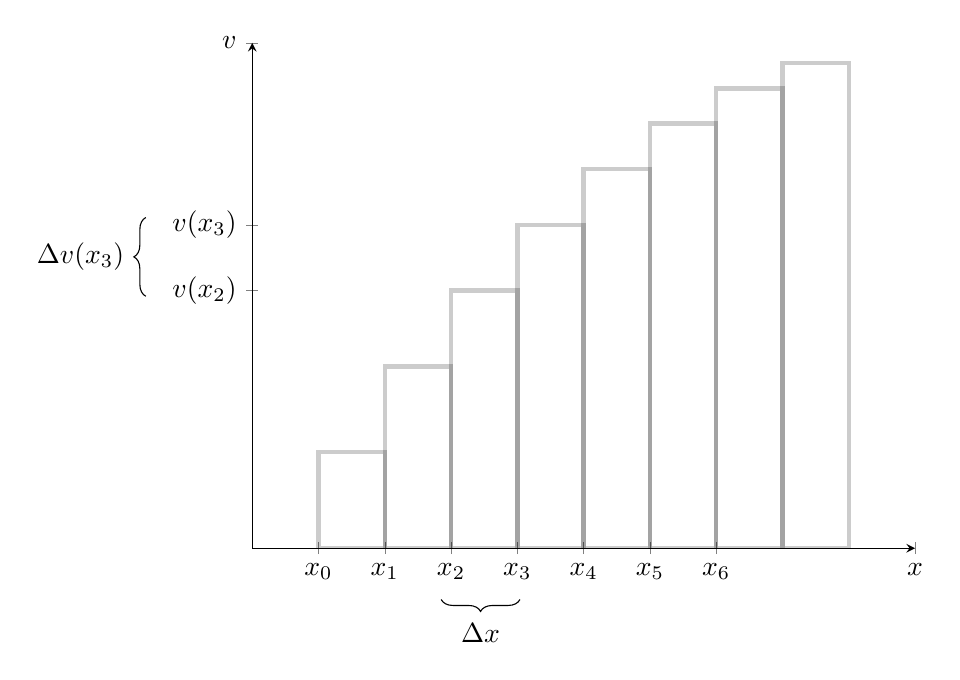
\begin{tikzpicture}[scale=1]
\begin{axis}[
  height=8cm, width=10cm,
axis x line=bottom, axis y line=left,
%   xlabel = Quantity $q$, ylabel = Utility $u$,
  ymin=0, ymax=.5, xmin=0, xmax=1,
  xtick={0.1, 0.2,0.3,0.4,0.5,0.6,0.7, 1},
  xticklabels={$x_0$,$x_1$,$x_2$,$x_3$,$x_4$,$x_5$,$x_6$,$x$,$q$},
  ytick={0.255, 0.32,.5},
  yticklabels={$v(x_2)$,$v(x_3)$,$v$},
]
    
%\addplot coordinates {(5, 5)} node[anchor=north] {$p^*$};

\node at (axis cs:12, 5) [anchor=south west] {A};
\node at (axis cs:20,11) [anchor=north west] {B};
%\addplot[color={rgb, 255:red, 74; green, 144; blue, 226 }, very thick,  domain=0:8, samples=1000, variable=\t]({t},  {t-t^2/2)} ) node[anchor=west] {$D(p)$} ;
%\addplot[color={rgb, 255:red, 226; green, 144; blue, 74 }, very thick,  domain=0:8, samples=1000, variable=\t]({t},  {t)} )node[anchor=west] {$S(p)$} ;
%\addplot[black, dashed,  domain=0:.3, samples=1000, variable=\t]({t},  {0.255}) )node[anchor=west] {$p$} ;
%\addplot[black, dashed,  domain=0:.4, samples=1000, variable=\t]({t},  {0.32}) )node[anchor=west] {$p$} ;


%\addplot[black, dashed,  domain=0:9, samples=1000, variable=\t]({t},  {5}) )node[anchor=west] {$p$} ;
% \draw [ultra thick, draw=black, fill=yellow, opacity=0.2]  (axis cs:0,0) -- (axis cs:5,5) -- (axis cs:0,5) -- cycle;
% \draw [ultra thick, draw=black, fill=none, opacity=0.2]  (axis cs:0,5) -- (axis cs:5,5) -- (axis cs:0,10) -- cycle;
%  \draw [ultra thick, draw=black, fill=none, opacity=0.2]  (axis cs:0.2,) -- (axis cs:5,5) -- (axis cs:0,10) -- cycle;
 \draw [ultra thick, draw=black, fill=none, opacity=0.2] (axis cs:0.1, 0) -- (axis cs:0.1, 0.095) -- (axis cs:0.2, 0.095) -- (axis cs:0.2, 0)-- cycle;
\draw [ultra thick, draw=black, fill=none, opacity=0.2] (axis cs:0.2, 0) -- (axis cs:0.2,0.18) -- (axis cs:0.3, 0.18) -- (axis cs:0.3, 0)-- cycle;
\draw [ultra thick, draw=black, fill=none, opacity=0.2] (axis cs:0.3, 0) -- (axis cs:0.3, 0.255) -- (axis cs:0.4,0.255) -- (axis cs:0.4, 0)-- cycle;
\draw [ultra thick, draw=black, fill=none, opacity=0.2] (axis cs:0.4, 0) -- (axis cs:0.4, 0.32) -- (axis cs:0.5, 0.32) -- (axis cs:0.5,0)-- cycle;
\draw [ultra thick, draw=black, fill=none, opacity=0.2] (axis cs:0.5, 0) -- (axis cs:0.5, 0.375) -- (axis cs:0.6, 0.375) -- (axis cs:0.6, 0)-- cycle;
\draw [ultra thick, draw=black, fill=none, opacity=0.2] (axis cs:0.6,0) -- (axis cs:0.6, 0.42) -- (axis cs:0.7, 0.42) -- (axis cs:0.7, 0)-- cycle;
\draw [ultra thick, draw=black, fill=none, opacity=0.2] (axis cs:0.7, 0) -- (axis cs:0.7,0.455) -- (axis cs:0.8, 0.455) -- (axis cs:0.8, 0)-- cycle;
\draw [ultra thick, draw=black, fill=none, opacity=0.2] (axis cs:0.8, 0) -- (axis cs:0.8, 0.48) -- (axis cs:0.9,0.48) -- (axis cs:0.9, 0)-- cycle;
% \draw [ultra thick, draw=black, fill=none, opacity=0.2] (axis cs:0.9, 0) -- (axis cs:0.9, 0.495) -- (axis cs:1., 0.495) -- (axis cs:1., 0)


\end{axis}
  \draw[decorate,decoration={brace,raise=1ex,amplitude=1ex}] (-1.2,3.2) -- (-1.2,4.2)
  node[midway,left=2ex] {$\Delta v(x_3)$};
  \draw[decorate,decoration={brace,raise=1ex,amplitude=1ex,mirror}] (2.4,-.5) -- (3.4,-.5)
  node[midway,below=2.2ex] {$\Delta x$};
 \end{tikzpicture}

\end{frame}


\end{document}